参见汪林《实分析中的反例》

\section{不同意义收敛的函数序列}

设 $\left\{f_n\right\}$ 是可测集 $E$ 上的 $p(1 \leqslant p<+\infty)$ 次幂 Lebesgue 可积函数序列,这时 $\left\{f_n\right\}$ 的收敛意义可以按多种意义解释。在这一章里,我们将考虑其中较常见的几种收敛意义,并指出它们之间的蕴涵关系,当没有蕴涵关系时就给出反例。我们要考虑的收敛意义是:

(1)\textbf{一致收敛}:$\lim _{n \rightarrow \infty} f_n(x)=f(x)$ 关于 $x \in E$ 一致地成立.

(2)\textbf{近一致收敛}:任给 $\delta>0$ ,存在 $E$ 的可测子集 $E_\delta$ ,使在 $E_\delta$ 上 $\left\{f_n\right\}$ 一致收敛于 $f$ ,而 $m\left(E \backslash E_\delta\right)<\delta$ .

(3)\textbf{几乎处处收敛} :$\lim _{n \rightarrow \infty} f_n(x)=f(x)$ 对于几乎所有的 $x \in E$ 成立.

(4)\textbf{测度收敛}:任给 $\varepsilon>0, \lim _{n \rightarrow \infty} m\left\{x:\left|f_n(x)-f(x)\right| \geqslant \varepsilon\right\}=0$ .

(5)\textbf{平均收敛}:
\[
\lim _{n \rightarrow \infty} \int_E\left|f_n(x)-f(x)\right|^p d x=0
\]
(6)弱收敛:
当 $1<p<+\infty$ 时,对每个 $g \in L^q(E), 1 / p+1 / q=1$ ,有
\[
\lim _{n \rightarrow \infty} \int_E f_n(x) g(x) d x=\int_E f(x) g(x) d x
\]
当 $p=1$ 时,对每个 $g \in L^{\infty}(E)$ ,有
\[
\lim _{n \rightarrow \infty} \int_E f_n(x) g(x) d x=\int_E f(x) g(x) d x
\]
\begin{remark}
凡是下面没有出现的蕴含关系,都存在反例!
\end{remark}
\subsection{\texorpdfstring{$E$}{E} 的测度有限时}

\begin{figure}[H]
\centering
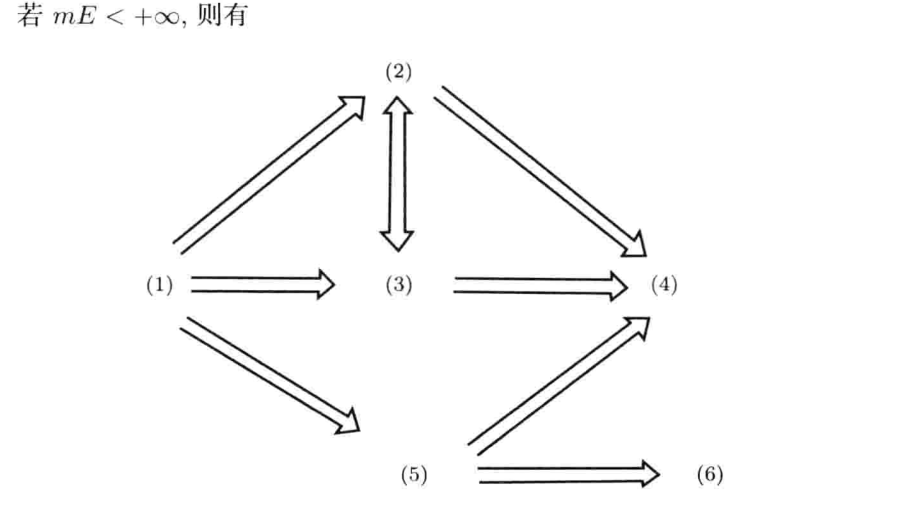
\includegraphics[width=\textwidth]{不同意义收敛的函数序列-2025040522.png}
% \caption{}
\label{}
\end{figure}

\subsection{\texorpdfstring{$E$}{E} 的测度无限时}

\begin{figure}[H]
\centering
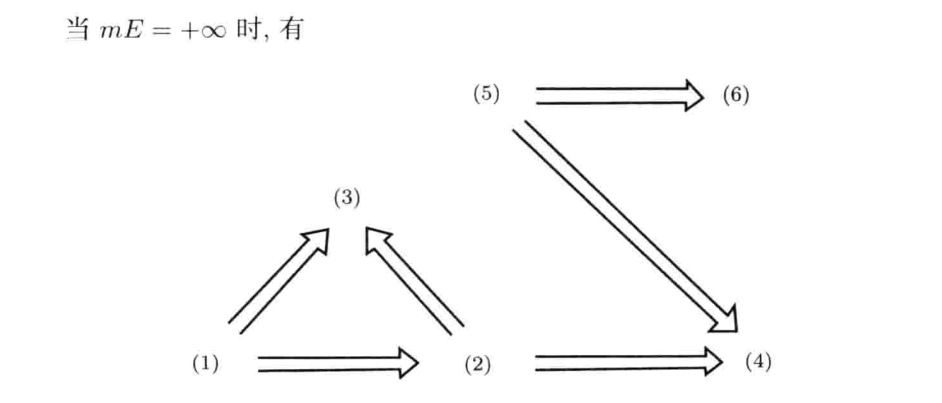
\includegraphics[width=\textwidth]{1-不同意义收敛的函数序列-2025040522.png}
% \caption{}
\label{}
\end{figure}
